\documentclass{article}

\title{Metodi Numerici per l'Informatica}
\author{Anthony}
\date{28 mar 2023}

\usepackage{amssymb}
\usepackage{amsmath}
\usepackage{graphicx}
\usepackage{algorithm}
\usepackage{algpseudocode}
\algnewcommand{\LeftComment}[1]{\Statex \(\triangleright\) #1}

\begin{document}
    \maketitle

    \section{Introduzione}
        Abbiamo preso familiarità con problemi lineari del tipo $\mathbf{Ax} = \mathbf{b}$ in cui $\mathbf{A}$ non è necessariamente 
        quadrata. Assumiamo da ora che $\mathbf{A}$ sia una matrice quadrata o alta, ovvero dispone abbastanza dati per risolvere il 
        sistema lineare. 
        \subsection{Spazio delle colonne}
            Possiamo scrivere $\mathbf{b}$ come combinazione lineare delle colonne di $\mathbf{A}$ con i coefficienti di $\mathbf{x}$:
            \[\mathbf{Ax} = \begin{pmatrix}
                \vline & \vline & \\
                \mathbf{a}_1 & \mathbf{a}_2 & \dots \\
                \vline & \vline & \\
            \end{pmatrix} \begin{pmatrix}
                x_1 \\
                x_2 \\
                \vdots
            \end{pmatrix} = x_1 \begin{pmatrix}
                \vline \\
                \mathbf{a}_1 \\
                \vline
            \end{pmatrix} + 
            x_2 \begin{pmatrix}
                \vline \\
                \mathbf{a}_2 \\
                \vline
            \end{pmatrix} + \dots\]
            Tutte le possibili combinazioni lineari di $\mathbf{A}$ formano lo \emph{spazio delle colonne}.
            \[\text{col }\mathbf{A} = \text{span}(\mathbf{a}_1, \mathbf{a}_2, \dots)\]
    \section{Instabilità numerica}
        Consideriamo il seguente problema:
        \[\mathbf{A} = \begin{pmatrix}
            \vline & \vline & \\
            \mathbf{a}_1 & \mathbf{a}_2 & \dots \\
            \vline & \vline & \\
        \end{pmatrix} = \begin{pmatrix}
            0 & 0.0001 & \\
            \vdots & \vdots & \dots \\
            1 & 1.0001 &
        \end{pmatrix}\]
        Le due colonne identificano due vettori quasi identici, cioè due vettori quasi paralleli. I vettori sono quasi linearmente 
        dipendenti. Se abbiamo un vettore $\mathbf{b}$ che è una combinazione lineare delle due colonne, esistono due modi che danno 
        approssimativamente un modo per esprimere $\mathbf{b}$. Questo ci porta a una situazione ambigua.
        \begin{center}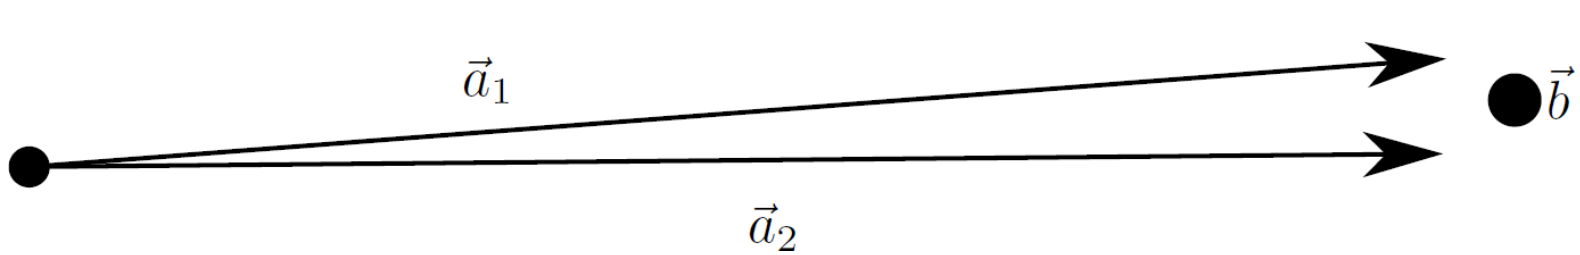
\includegraphics[width=10cm]{almost_dependant.png}\end{center}
        \[\mathbf{b} \approx x_1\mathbf{a}_1 + x_2\mathbf{a}_2\]
        \[\mathbf{b} \approx x_2\mathbf{a}_1 + x_1\mathbf{a}_2\]
        Questo problema si dice \emph{malcondizionato} per via dell'\emph{instabilità numerica} dei due vettori quasi-paralleli. \\
        In generale, una soluzione per un problema del tipo $\mathbf{Ax}=\mathbf{b}$ potrebbe non esistere o essere unica e dipende proprio 
        dallo spazio delle colonne di $\mathbf{A}$ per cui vogliamo risolvere il problema dell'instabilità numerica.
    
    \section{Ortogonalità}
        Consideriamo due vettori $\mathbf{a}$ e $\mathbf{b}$. Supponiamo di voler proiettare $\mathbf{b}$ verso $\mathbf{a}$. 
        \begin{center}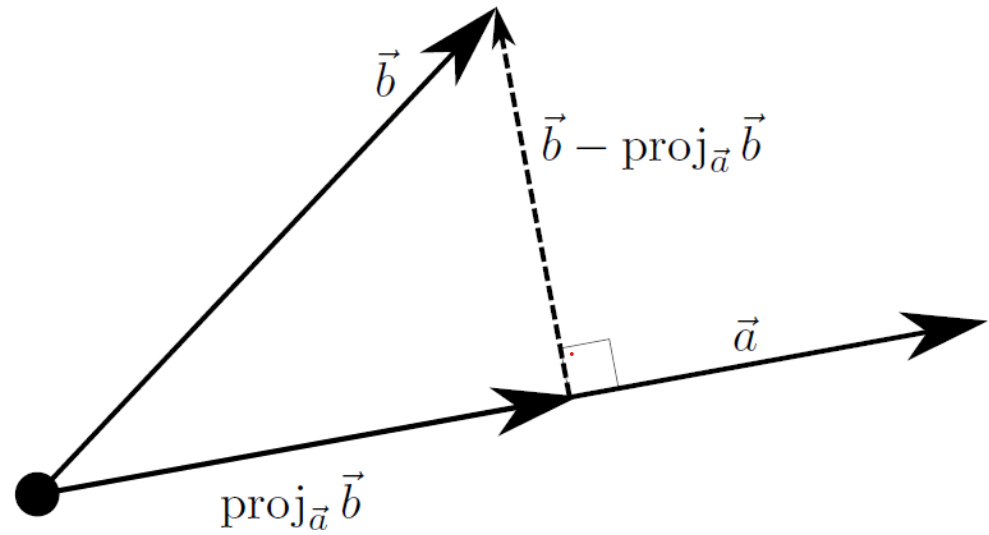
\includegraphics[width=8cm]{projection.png}\end{center}
        Tale proiezione possiamo vederla come un multiplo di $\mathbf{a}$, per cui possiamo chiederci per quale scalare $c$ il vettore
        $\mathbf{a}$ è il più vicino a $\mathbf{b}$:
        \[\min_c \Vert c \cdot \mathbf{a} - \mathbf{b} \Vert_2^2 \]
        Sia tale scalare $c^*$, esso rappresenta la proiezione di $\mathbf{b}$ su $\mathbf{a}$:
        \[ \text{proj}_\mathbf{a}\mathbf{b} \equiv c^*\mathbf{a}\] 
        Possiamo osservare che il \emph{complemento} $\mathbf{b} - \text{proj}_\mathbf{a}\mathbf{b}$ è \emph{ortogonale} a $\text{proj}_\mathbf{a}\mathbf{b}$. 
        Tale vettore si chiama \emph{complemento ortogonale}.\\
        Il problema della proiezione equivale a trovare una soluzione ai minimi quadrati in cui $\mathbf{a}\cdot c \approx \mathbf{b}$. Possiamo 
        applicare la stessa soluzione che abbiamo già visto in precedenza: calcoliamo il gradiente, lo poniamo uguale a zero e risolviamo per $c$.
        \[c = \frac{\mathbf{a}^T\mathbf{b}}{\mathbf{a}^T\mathbf{a}}\]
        Osserviamo che al numeratore non abbiamo altro che la norma $\ell_2$:
        \[c = \frac{\mathbf{a}^T\mathbf{b}}{\Vert \mathbf{a} \Vert_2^2}\]
        Per cui
        \[ \text{proj}_\mathbf{a}\mathbf{b} = \frac{\mathbf{a}^T\mathbf{b}}{\Vert \mathbf{a} \Vert_2^2}\]

        In maniera analoga, possiamo proiettare $\mathbf{b}$ su un intero spazio vettoriale. Assumiamo di avere una base \emph{ortonormale} $\{\mathbf{a}_1,\dots,\mathbf{a}_k\}$,
        ovvero una base in cui 
        tutti i vettori sono perpendicolari e con norma pari a 1,
        allora possiamo proiettare un vettore sul suo span risolvendo il problema:
        \[ \min_{c_1,\dots,c_k} \Vert c_1\mathbf{a}_1 + \dots + c_k\mathbf{a}_k - \mathbf{b} \Vert_2^2\]
        \paragraph{Esempio} Assumiamo di essere in $\mathbb{R}^3$ con $k=2$:
        \begin{center}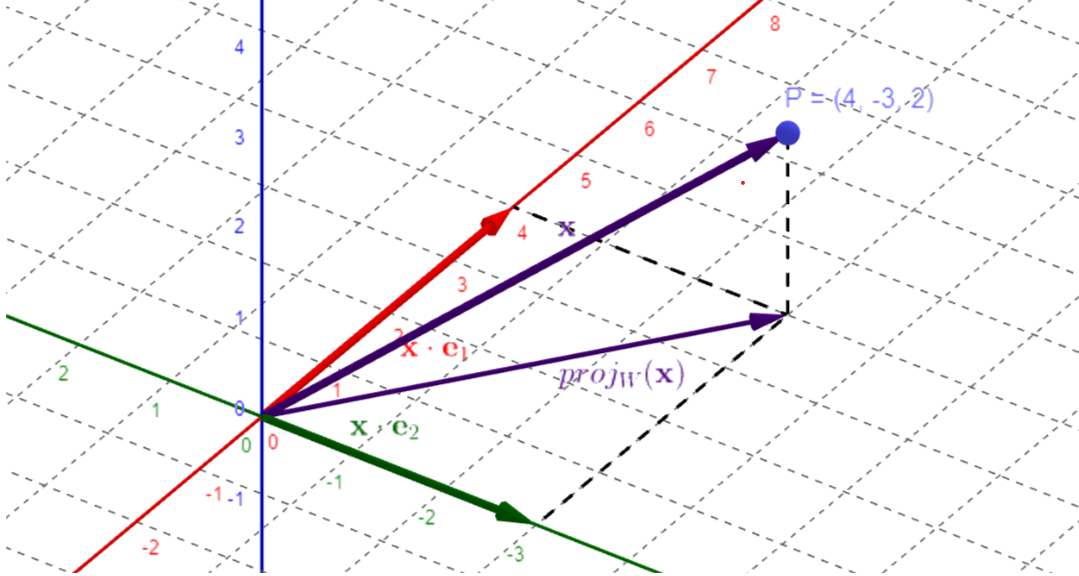
\includegraphics[width=8cm]{proj_on_plane.png}\end{center}
        La soluzione è analoga a prima, ma anziché risolvere per uno scalare risolviamo per $k$ scalari. Il problema della proiezione si 
        risolve quindi come segue:
        \[ \text{proj}_{\text{span}(\mathbf{a}_1, \dots, \mathbf{a}_k)} \mathbf{b} = (\mathbf{a}_1^T\mathbf{b})\mathbf{a}_1 + \dots + (\mathbf{a}_k^T \mathbf{b})\mathbf{a}_k\]
        \textbf{Oss:} non dividiamo per la norma perché abbiamo assunto una base ortonormale.

        \subsection{Matrici ortogonali}
            Abbiamo finora esplorato due concetti, ortogonalità e ortonormalità:
            \begin{itemize}
                \item Due vettori si dicono ortogonali se l'angolo che formano è di 90 gradi;
                \item Due vettori sono ortonormali se sono ortogonali e se hanno norma pari a 1.
            \end{itemize}
            Una matrice si dice \emph{ortogonale} se le sue colonne sono ortonormali. Osserviamo ora il seguente problema banale:
            \[\mathbf{Ix} = \mathbf{b}\]
            In cui $\mathbf{I}$ è la matrice identica. La soluzione ovvia del problema è $\mathbf{x} = \mathbf{b}$. Abbiamo già osservato che 
            l'errore dei minimi quadrati $\mathbf{Ax} \approx \mathbf{b}$ corrisponde al seguente problema lineare:
            \[\mathbf{A}^T\mathbf{Ax} = \mathbf{A}^T\mathbf{b}\]
            Sia $\mathbf{A}$ una matrice ortogonale, abbiamo che $\mathbf{AA}^T = \mathbf{I}$, per cui ricadiamo nel caso banale.\\
            Per chiarezza ora, indichiamo con $\mathbf{Q}$ una generica matrice ortogonale. Il prodotto $\mathbf{Q}^T\mathbf{Q}$ ha la forma:
            \[\mathbf{Q}^T\mathbf{Q} = \begin{pmatrix}
                - & \vec{q}_1^T & - \\
                - & \vec{q}_2^T & - \\
                & \vdots & \\
                - & \vec{q}_n^T & - \\
            \end{pmatrix} \begin{pmatrix}
                \vline & \vline & & \vline \\
                \vec{q}_1 & \vec{q}_2 & \dots & \vec{q}_n \\
                \vline & \vline & & \vline
            \end{pmatrix} = \begin{pmatrix}
                \vec{q}_1 \cdot \vec{q}_1 & \vec{q}_1 \cdot \vec{q}_2 & \dots & \vec{q}_1 \cdot \vec{q}_n \\
                \vec{q}_2 \cdot \vec{q}_1 & \vec{q}_2 \cdot \vec{q}_2 & \dots & \vec{q}_2 \cdot \vec{q}_n \\
                \vdots & \vdots & \dots & \vdots \\
                \vec{q}_n \cdot \vec{q}_1 & \vec{q}_n \cdot \vec{q}_2 & \dots & \vec{q}_n \cdot \vec{q}_n \\
            \end{pmatrix}\]
            Osserviamo che la diagonale contiene tutte le lunghezze al quadrato delle colonne di $\mathbf{Q}$. 
            Tutte le colonne di $\mathbf{Q}$ sono ortogonali e hanno lunghezza 1 per cui $\mathbf{Q}^T\mathbf{Q} = \mathbf{I}$. Se le colonne 
            di $\mathbf{Q}$ non avessero lunghezza 1, sulla diagonale avremmo solo i quadrati delle lunghezze delle colonne. 
            Le colonne di $\mathbf{Q}$ formano una base ortonormale per lo spazio delle colonne. \\
            Esempi:
            \begin{enumerate}
                \item La base standard è una base ortonormale.
                \item La matrice identità $\mathbf{I}$ è ortogonale.
                \item Qualsiasi matrice di permutazione, ovvero una matrice che ha un unico 1 su ogni colonna e su ogni riga e 0 altrove, 
                 è ortogonale.
            \end{enumerate}


            \subsubsection{Isometria}
                Le matrici ortogonali, in quanto matrici, modellano delle mappe lineari. Le matrici ortogonali hanno la proprietà che,
                quando applicate a un vettore, la lunghezza del vettore non cambia:
                \[ \Vert \mathbf{Qx} \Vert_2^2 = \mathbf{x}^T \mathbf{Q}^T \mathbf{Qx} = \mathbf{x}^T \mathbf{I}\mathbf{x} = \mathbf{x}^T \mathbf{x} = \Vert \mathbf{x} \Vert_2^2\]
                Le matrici ortogonali, inoltre, preservano l'angolo tra due vettori (prodotto interno):
                \[ \langle \mathbf{Qx},\mathbf{Qy} \rangle = \mathbf{x}^T \mathbf{Q}^T\mathbf{Qy} = \mathbf{x}^T \mathbf{I} \mathbf{y} = \mathbf{x}^T\mathbf{y}\]
                Per queste proprietà, la mappa $\mathbf{x} \mapsto \mathbf{Qx}$ è un \emph{isometria} in $\mathbb{R}^n$, ovvero rappresenta 
                una rotazione dello spazio.
                \begin{center}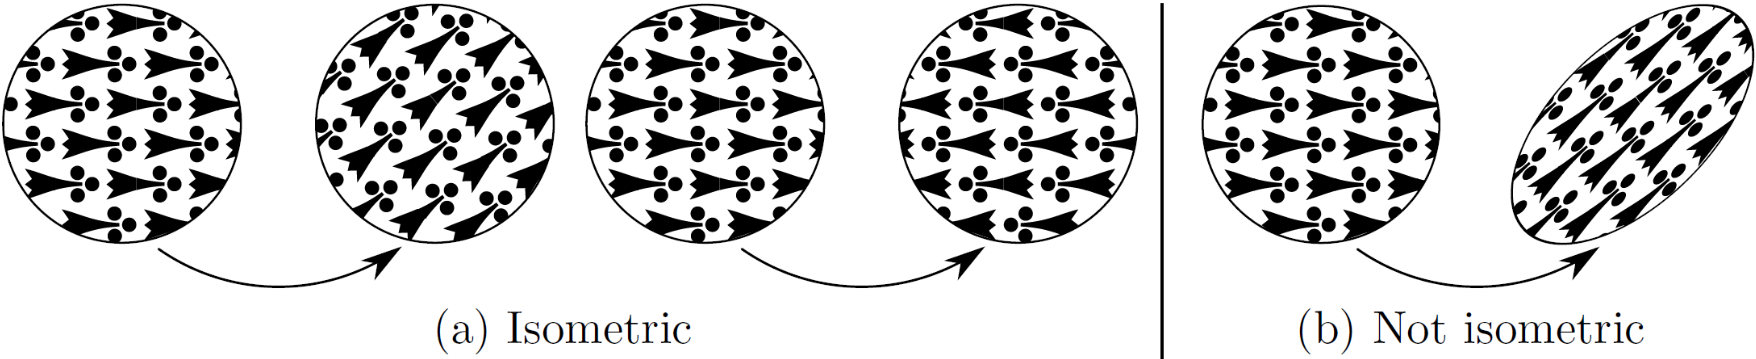
\includegraphics[width=12cm]{isometric.png}\end{center}

        \subsection{Matrici non ortogonali}
            Quando risolviamo un problema del tipo $\mathbf{Ax} = \mathbf{b}$, tipicamente $\mathbf{A}$ non è ortogonale, 
            le matrici ortogonali, tuttavia, possono aiutarci a semplificare il problema. \\
            Idea: possiamo riscrivere $\mathbf{A}$ come prodotto di due matrici tali che $\mathbf{A}^T\mathbf{Ax} = \mathbf{A}^T\mathbf{b}$ 
            è più facile da risolvere. In particolare, supponiamo che possiamo scrivere la matrice $\mathbf{A}$ come segue:
            \[\mathbf{A} = \mathbf{QR}\]
            In cui $\mathbf{Q}$ è ortogonale e $\mathbf{R}$ è invertibile. Per cui l'operazione
            \[\mathbf{AR}^{-1} = \mathbf{Q}\]
            data la matrice $\mathbf{A}$, la trasformiamo attraverso la matrice $\mathbf{R}^{-1}$ e ciò fa sì che le colonne di $\mathbf{A}$
            diventino ortogonali. Questo significa che possiamo ortogonalizzare qualunque matrice.

    \section{Decomposizione QR}
        Qualsiasi matrice $\mathbf{A}$ ammette la fattorizzazione:
        \[\mathbf{A} = \mathbf{QR} \]
        Ciò significa che possiamo ortogonalizzare le colonne di $\mathbf{A}$. Inoltre, lo spazio delle colonne di $\mathbf{A}$ è
        identico allo spazio delle colonne di $\mathbf{AR}^{-1}$:
        \[ \text{col } \mathbf{AR}^{-1} = \text{col } \mathbf{A}\]
        Ciò ci suggerisce che ortogonalizzare le colonne di $\mathbf{A}$ non cambia lo spazio che esse spannano. Dato che $\mathbf{Q}=\mathbf{AR}^{-1}$
        possiamo affermare che:
        \[\text{col }\mathbf{Q} = \text{col }\mathbf{A}\]
        Per cui le colonne di $\mathbf{Q}$ formano una base ortonormale per le $\text{col }\mathbf{A}$.
        
        \subsection{Colonne quasi-parallele}
            Riprendendo l'esempio delle colonne \emph{quasi parallele}:
            \[\mathbf{A} = \begin{pmatrix}
                \vline & \vline & \\
                \mathbf{a}_1 & \mathbf{a}_2 & \dots \\
                \vline & \vline & \\
            \end{pmatrix} = \begin{pmatrix}
                0 & 0.0001 & \\
                \vdots & \vdots & \dots \\
                1 & 1.0001 &
            \end{pmatrix}\]

            Con l'ortogonalizzazione possiamo condizionare meglio il problema.
            \begin{center}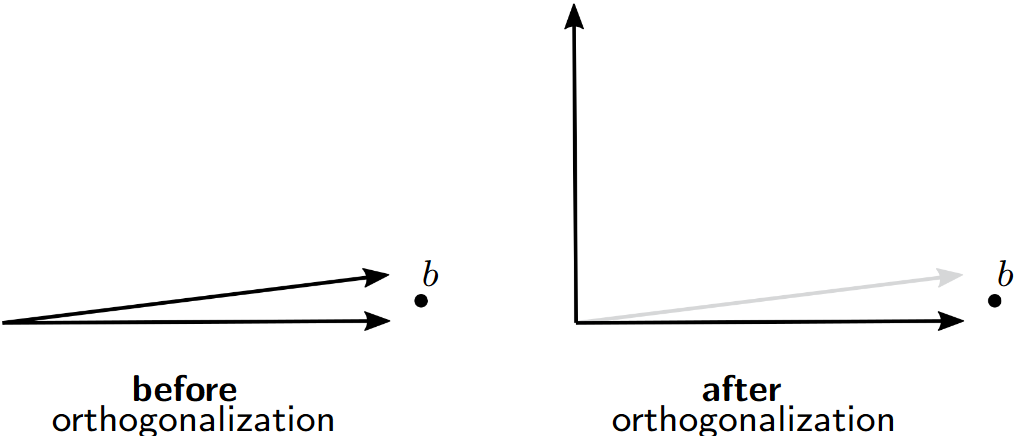
\includegraphics[width=10cm]{quasi_par.png}\end{center}
            Usando la fattorizzazione QR, l'equazione
            \[\mathbf{A}^T\mathbf{Ax} = \mathbf{A}^T\mathbf{b}\]
            Diventa:
            \[ ( \mathbf{QR} )^T \mathbf{QRx} = (\mathbf{QR})^T \mathbf{b} \]
            \[ = \mathbf{R}^T \mathbf{Q}^T \mathbf{QRx} = \mathbf{R}^T \mathbf{Q}^T \mathbf{b} \]
            \[ = \mathbf{R}^T \mathbf{IRx} = \mathbf{R}^T \mathbf{Q}^T \mathbf{b}\]
            \[ = \mathbf{Rx} = \mathbf{Q}^T\mathbf{b} \quad \text{per invertibilità di $\mathbf{R}$}\] 
            Un'altra proprietà della matrice $\mathbf{R}$ è che è \emph{triangolare superiore}. Ciò rende il problema più 
            facile da risolvere con la \emph{back-substitution}.

        \subsection{Algoritmo Gram-Schmidt}
            L'algoritmo, dati due vettori $\vec{v_1}, \vec{v_2}$, attraverso le proiezioni ortogonali, ortogonalizza i due vettori.
            \begin{center}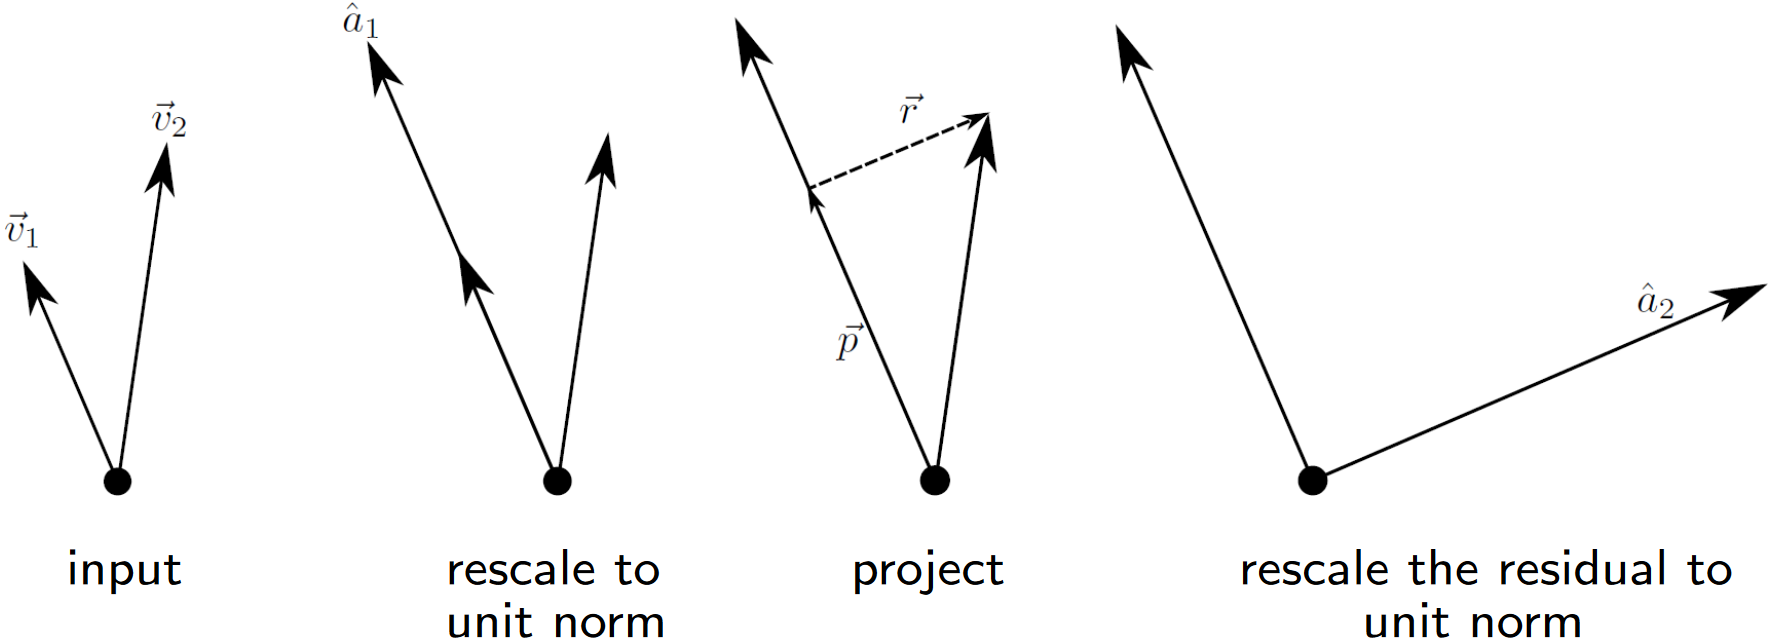
\includegraphics[width=10cm]{gram_schmidt_vects.png}\end{center}
            Possiamo osservare che:
            \begin{enumerate}
                \item I vettori ortogonalizzati spannano lo stesso spazio di $\vec{v_1}$ e $\vec{v_2}$
                \item L'algoritmo funziona in modo incrementale: possiamo ortogonalizzare un qualsiasi numero di vettori uno alla volta
                \item Se i vettori in input sono le colonne di $\mathbf{A}$, i vettori in output ortogonalizzati sono le colonne di $\mathbf{Q}$. Per ottenere $\mathbf{R}$,
                 possiamo computare semplicemente $\mathbf{R} = \mathbf{Q}^T\mathbf{A}$
            \end{enumerate}

            Osserviamo ora l'implementazione in pseudo-codice dell'algoritmo di Gram-Schmidt. Ricordiamo che il residuo non è altro che 
            il complemento ortogonale.
            \begin{algorithm}
                \caption{Gram-Schmidt}
                \label{Gram-Schimdt}
                \begin{algorithmic} % The number tells where the line numbering should start
                    \Function{Gram-Schmidt}{$\vec{v_1}, \vec{v_2}, \dots, \vec{v_k}$}
                        \LeftComment{Assume che $\vec{v_1}, \vec{v_2}, \dots, \vec{v_k}$ sono linearmente indipendenti.}
                        \LeftComment{Trova una base ortonormale $\hat{a_1}, \dots, \hat{a_k}$ per $\text{span }\{\vec{v_1}, \vec{v_2}, \dots, \vec{v_k}\} $}
                        \State $\hat{a_1} \gets \vec{v_1}/\Vert \vec{v_1} \Vert_2$ \Comment{Scaliamo il primo vettore}
                        \For{$i \gets 2,3, \dots, k$}
                            \State $\vec{p} \gets \vec{0}$
                            \For{$j \gets 1,2, \dots, i-1$} \Comment{Proiezione di $\vec{v_i}$ sullo $\text{span }\{\hat{a_1}, \dots, \hat{a_{i-1}}\}$ }
                                \State $\vec{p} \gets \vec{p} + (\vec{v_i} \cdot \hat{a_j})\hat{a_j}$ \Comment{Proiezione sulla base ortonormale}
                            \EndFor
                            \State $\vec{r} \gets \vec{v_i} - \vec{p}$ \Comment Il residuo è ortogonale alla base corrente
                            \State $\hat{a_i} \gets \vec{r}/\Vert \vec{r} \Vert_2$ \Comment Normalizziamo il residuo e aggiungiamolo alla base
                        \EndFor
                        \State \Return $\{ \hat{a_1}, \dots, \hat{a_k}\}$
                    \EndFunction
                \end{algorithmic}
            \end{algorithm}

            \subsection{Varianti di Gram-Schmidt}
                Nel problema $\mathbf{Ax} = \mathbf{b}$ sappiamo che $\mathbf{A}$ potrebbe essere rettangolare, in particolare alta. 
                Supponiamo essa abbia dimensioni $m \times n$. Che forma devono avere $\mathbf{Q}$ ed $\mathbf{R}$?
                \[\underbrace{\mathbf{A}}_{m \times n} = \underbrace{\mathbf{Q}}_{m \times n} \underbrace{\mathbf{R}}_{n \times n}\]
                oppure
                \[\underbrace{\mathbf{A}}_{m \times n} = \underbrace{\mathbf{Q}}_{m \times m} \underbrace{\mathbf{R}}_{m \times n}\]
                Questo ci suggerisce che esistono due fattorizzazioni valide per $\mathbf{A}$. In una $\mathbf{R}$ è quadrata, 
                mentre nell'altra $\mathbf{Q}$ è quadrata. L'algoritmo Gram-Schimdt standard implementa la prima equazione, ovvero 
                quella in cui $\mathbf{R}$ è quadrata. Ci sono altre varianti che implementano la seconda equazione, ma dobbiamo osservare che 
                se $\mathbf{Q}$ è quadrata, e $m > n$, ovvero $\mathbf{A}$ è alta, allora significa che $\mathbf{Q}$ ha più colonne 
                di quante ne avevamo in $\mathbf{A}$. Tali colonne, le ultime $n-k$, possono essere ignorate. 
                Esistono diverse varianti dell'algoritmo Gram-Schmidt ed essi barattano l'efficienza per lo spazio e viceversa.
\end{document}